\documentclass{standalone}
\usepackage{tikz}
\usetikzlibrary{matrix, positioning}

\begin{document}
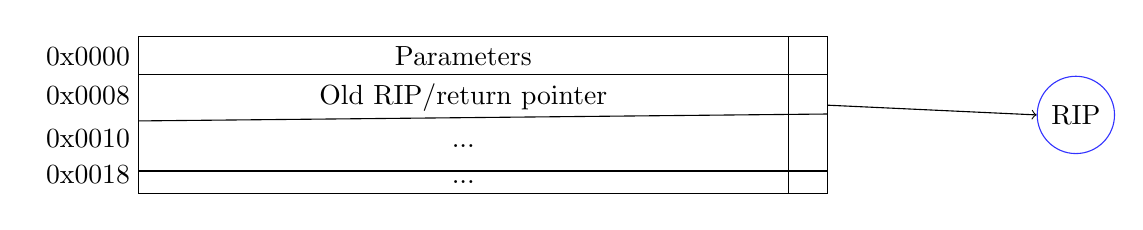
\begin{tikzpicture}

\matrix (m) [matrix of nodes, nodes in empty cells,
column sep=0, row sep=0,
column 1/.style={},
column 2/.style={nodes={text width=8cm, align=center}},
column 3/.style={nodes={minimum width=5mm}}] {

0x0000	& Parameters &\\
0x0008	& Old RIP/return pointer & \\
0x0010	& ... &\\
0x0018	& ... & \\
};

\draw node (n) [circle, draw=blue!80, right=1in of m]{RIP};
\draw[->] (m-2-3) -- (n.west);
\draw (m-1-2.north west) rectangle (m-4-2.south east);
\draw (m-1-2.north east) rectangle (m-4-3.south east);
\draw (m-4-2.north west) rectangle (m-4-2.south east);
\draw (m-4-2.north east) rectangle (m-4-3.south east);

\foreach \x in {1, 2} {
\draw (m-\x-2.south west) -- (m-\x-3.south east);
};

\end{tikzpicture}
\end{document}